\documentclass[a4paper,11pt]{article}

% set up sensible margins (same as for cssethesis)
\usepackage[paper=a4paper,left=30mm,right=30mm,top=25mm,bottom=25mm]{geometry}
\usepackage{natbib} % Use the natbib bibliography and citation package
\usepackage{setspace} % This is used in the title page
\usepackage{graphicx} % This is used to load the crest in the title page
\usepackage{physics} % Used for \abs

% non-template packages
\usepackage{paralist}
\usepackage{multicol}
\usepackage{caption}
\usepackage{tabularx, booktabs}
\newcolumntype{Y}{>{\centering\arraybackslash}X}
\usepackage{listings}
\lstset{
	numbers=left, 
	numberstyle=\small, 
	numbersep=8pt, 
	frame = single, 
	language=Python, 
	framexleftmargin=17pt}

\usepackage{tikz}
\usepackage{smartdiagram}

\usepackage[font={small,it}]{caption}
\usepackage{hyperref}
\usepackage{xcolor}
\usepackage{lscape}
\hypersetup{
	colorlinks,
	linkcolor=teal,
	citecolor=teal,
	urlcolor=blue
}

\usepackage[english]{babel}
\usepackage{blindtext}
\usepackage{footnote}
\makesavenoteenv{tabular}
\makesavenoteenv{table}

%tikz stuff
\usepackage{tikz}
\usetikzlibrary{shapes, arrows, trees}
\tikzstyle{decision} = [diamond, draw, fill=green!20, text width=4.5em, text badly centered, node distance=3cm, inner sep=0pt]
\tikzstyle{block} = [rectangle, draw, fill=yellow!20, text width=3cm, text centered, rounded corners, minimum height=4em]
\tikzstyle{line} = [draw, -latex']
\tikzstyle{straight} = [draw]


\usepackage{array}
\newcolumntype{L}[1]{>{\raggedright\let\newline\\\arraybackslash\hspace{0pt}}m{#1}}
\newcolumntype{C}[1]{>{\centering\let\newline\\\arraybackslash\hspace{0pt}}m{#1}}
\newcolumntype{R}[1]{>{\raggedleft\let\newline\\\arraybackslash\hspace{0pt}}m{#1}}

\usepackage{float}

%\hypersetup{
%	colorlinks,
%	linkcolor={red!50!black},
%	citecolor={blue!50!black},
%	urlcolor={blue!80!black}
%}

\begin{document}
	
% Set up a title page
\thispagestyle{empty} % no page number on very first page
% Use roman numerals for page numbers initially
\renewcommand{\thepage}{\roman{page}}

\begin{spacing}{1.5}
	\begin{center}
		{\Large \bfseries
			School of Computer Science (BICA) \\
			Monash University}
		
		
		\vspace*{30mm}
		
		
\includegraphics[width=5cm]{graphics/MonashCrest.pdf}
		
		\vspace*{15mm}
		
		{\large \bfseries
			Literature Review, 2017
		}
		
		\vspace*{10mm}
		
		{\LARGE \bfseries
			Review of optimal multi-agent pathfinding algorithms and usage in warehouse automation
		}
		
		\vspace*{20mm}
		
		{\large \bfseries
			Phillip Wong
			
			\vspace*{20mm}
			
			
			Supervisors: \parbox[t]{50mm}{Daniel Harabor,\\Pierre Le Bodic}
		}
		
	\end{center}
\end{spacing}

\newpage

\tableofcontents

\newpage
% Now reset page number counter,and switch to arabic numerals for remaining
% page numbers 
\setcounter{page}{1}
\renewcommand{\thepage}{\arabic{page}}

\section{Introduction} \label{sec:introduction}
% What
The order picking process is the number one expense in the operating cost of warehouse systems (\cite{de2007design}). Order picking involves the retrieval of inventory from around the warehouse.
This project looks at the use of multi-agent pathfinding (MAPF) algorithms within order picking. In particular, we explore Kiva systems (\cite{wurman2008coordinating}) where the order-picking process is performed by autonomous vehicles.

Firstly we define the components making up a Kiva system (Figure~\ref{fig:kivaprocess}). \textit{Drive units} are our autonomous vehicles which move around the warehouse, retrieving and delivering shelving units. These shelving units are known as \textit{storage pods} and are usually organized in aisles. Lastly we have the \textit{picking station} where a human workers are situated. With these defined, the process of order picking in a Kiva system is as follows:
\begin{compactenum}
	\item An order is received requesting one or more products
	\item The system identifies storage pods containing the said products
	\item The system schedules drive units to pickup the storage pods
	\item Once a drive unit is ready, it will move to the storage pod, pick it up and deliver it to the correct picking station
	\item Once the drive unit has delivered the storage pod, a human worker situated at the picking station will pick the product off the storage pod and pack it into a box
	\item After the storage pod has been picked, the drive unit agent returns it to a suitable location
	\item Finally once all the products for the order have been packed, the box it is processed and sent off
\end{compactenum}


%\noindent There are a number of related and inter-dependent optimization problems which make this process especially challenging. For example, step (1)  requires that the system prioritize the requests and assign each one to a pick station; step (3) involves matching requests to drive units; steps (4) and (6) involves coordinating the drive units. There are also additional considerations to further complicate things. These include requests that can only be satisfied by products from several different shelving units (and which are possibly serviced by multiple drive units), product replenishment and the drive units themselves having a limited battery capacity.


\noindent As this process describes, Kiva systems have a number of inter-dependent problems to solve. step 1. requires that the system assigns an order to a picking station; step 3. involves identifying a suitable drive unit to picking a storage pod. Other notable areas include: the replenishment requirement for the batteries of drive units and the products stored in the storage pods; a robotics problem described in the Amazon picking challenge (\cite{correll2016lessons}) which aims to make the picking process autonomous.

\begin{figure}[h!]
	\centering
	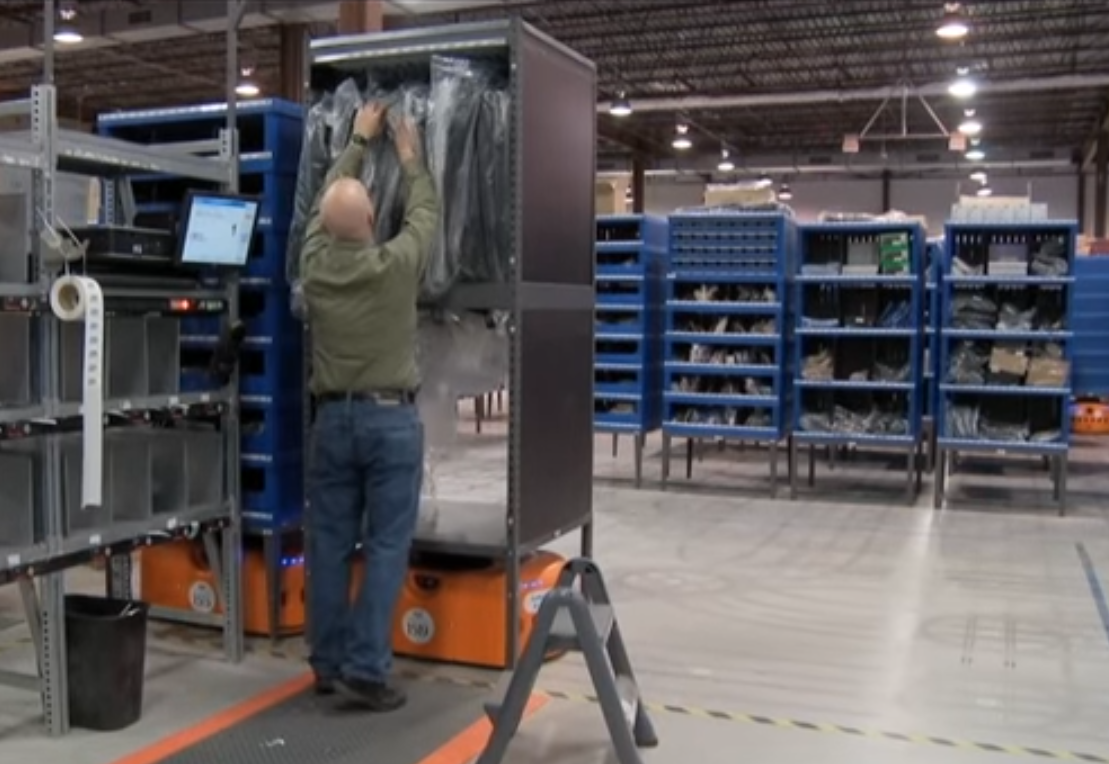
\includegraphics[width=0.6\textwidth ]{graphics/kivaprocess}
	\caption{A worker picking an order from a storage pod. The orange robot underneath is the drive unit. (\cite{kivayoutube2010quietlogistics})}
	\label{fig:kivaprocess}
\end{figure}

Solving all these problems and applying them in one solution has been done by the creators of Kiva systems but is unfortunately is not described in any literature. The consequences of optimizing these systems together would be very useful but is out of the scope of this project. Here we will be focusing on heart of the order-picking process which is the MAPF problem.


We see that a MAPF problem arises when a drive unit agent retrieves, delivers or returns a storage pod (steps 4 and 6). Here we need a solution to coordinate drive unit agents so they can move around the warehouse while avoiding collisions. This is not a simple task as solving MAPF optimally is an NP-hard problem (\cite{yu2013structure}). We can conclude that Kiva systems in production are using a suboptimal algorithms as these warehouses run over 1000 agents. This forms the motivation behind our project, to look at the benefits we may find in Kiva systems by using an optimal approach and what we will have to sacrifice for scalability. Later in Section~\ref{sec:optimal}, we look at the performance of these optimal algorithms.

Our main contribution in this literature review is comparing the scalability of optimal and suboptimal MAPF algorithms and seeing how past work has tried to bridge this gap. Additionally, we look at any algorithms which were applied to a Kiva system setting; what simplifications they assumed and what conclusions they have drawn to the usability. 

% How
Section~\ref{sec:background} describes in detail, the MAPF problem and according terminology. Section~\ref{sec:problemdef} formally outlines the Kiva system problem. Section~\ref{sec:suboptimal} describes some state-of-the-art suboptimal MAPF algorithms. Section~\ref{sec:optimal} looks at optimal MAPF algorithms. Section~\ref{sec:generalimprovements} looks at \textit{operator decomposition} and \textit{independence detection}. Finally, Section~\ref{sec:discussion} discusses the findings of this literature review, identifying possible research gaps in improving scalability and applications to Kiva systems.

%In order to find an optimal solution we will be using formulating the MAPF problem as a mixed integer program. Section~\ref{sec:optimal} will look at past approaches taken to MAPF.
% Why
%The aim of this literature review is to summarize the state-of-the-art in optimal MAPF, compare them to the scalability of suboptimal algorithms and identify which algorithms have been tested in a Kiva system environment.

\section{Background} \label{sec:background}
\subsection{Single-agent pathfinding} 
The single-agent pathfinding problem aims to find a path from start node to goal node. A detailed review of single agent search algorithms can be found in the \textit{grid-based path planning competition} (\cite{sturtevant2015grid}). The paper overviews all the entries to the competition and their relative performance. The algorithms are run on a number of game maps from \cite{sturtevant2012benchmarks} which are used for benchmarking and these maps are also used in many MAPF benchmarks. The results from \cite{sturtevant2015grid} are a few years old but we are expecting new approaches from this year's GPPC.

In this project, we aim to look at two single-agent search algorithms: \textit{jump point search} (\cite{harabor2011online}) and \textit{compressed path databases} (\cite{strasser2015compressing}).

\subsection{Multi-agent pathfinding} In this section, we describe the problem of \textit{multi-agent pathfinding} (MAPF). The MAPF problem is a generalization of the single-agent pathfinding problem for multiple agents and single agent pathfinding algorithms are often used a sub-solver within the MAPF algorithm. The task of MAPF is to coordinate a number of agents moving around an environment. Each agent must find a path to their goal while ensuring that no agent collides with another. A common secondary objective is to minimize either the makespan of the system or the sum of costs. As mentioned in Section~\ref{sec:introduction}, solving MAPF optimally is an NP-hard problem (\cite{yu2013structure}). Suboptimal and optimal MAPF have vastly different properties in scalability and solution quality. Thus they are compared in different sections [\ref{sec:suboptimal}, \ref{sec:optimal}] of this literature review. Later in Section~\ref{sec:problemdef} we formally define the MAPF problem in the context of Kiva systems.

Below are some important properties of MAPF algorithms. Table~\ref{table:comparison} shows a comparison of these properties across the all MAPF algorithms discussed in this literature review.

\noindent \textbf{Completeness:} A complete algorithm will always return valid solution to the MAPF problem if one exists.

\noindent \textbf{Solution quality:} Solution quality is usually measured in makespan or sum of costs. Makespan is the number of timestep required from the start state to the goal state where all agents are at their goals. Sum of costs is the sum of the number of timesteps taken for each individual agent to reach their goal.
\begin{compactitem}
	\item Optimal: finds the optimal path to the goal minimizing the objective
	\item Bounded suboptimal: given a optimal path cost of $C$, the cost of a bounded suboptimal solution, $B$ is guaranteed to be within $C$ and $w*C$ where $w$ is a user set parameter. Hence, $C \le B \le wC$.
	\item Suboptimal: finds a path to the goal with no guarantee of solution cost
\end{compactitem}

\noindent \textbf{Anytime:} The search can spend more computation to improve the solution quality or number of solutions, it can stop earlier at any time and return a path.

\noindent \textbf{Centralized / Coupled:} In a centralized approach, all agents are looked at globally and a decision is made with all paths in mind. In a decentralized approach, paths are found for one agent at time. A centralized approach is usually has the properties of an optimal solution and is not scalable. Accordingly, a decentralized approach scales up to many agents but is suboptimal and often non-complete.

\noindent \textbf{Success rate:} Success rate is often used as a measure of performance for optimal algorithms. It describes the percentage of instances which were capable of being solved within a fixed time $t$, usually set at 5 minutes.

\subsection{Bounded-suboptimal variants} \label{sec:bsov}
A \textit{bounded suboptimal variant} is a variant of an optimal MAPF algorithm. The defining feature of a bounded suboptimal variant is that we are able to guarantee that the cost of the bounded suboptimal solution, $B$ lies within the optimal cost $C$ and $w*C$ where $w$ is a user-defined parameter. A bounded suboptimal variant provides a way of trading speed for solution quality and is especially relevant this project as we want to find a middle ground between optimality and speed Kiva systems. The optimal algorithms in \ref{sec:optimal} will mention any bounded suboptimal variants if they exist.

%\noindent \textbf{Integer Linear Programming}. Integer Linear Programming (ILP) is an optimization technique. It looks at an objective function subject to a list of constraints and finds the optimal solution for each variable. \textbf{not sure what to write here?}

%\[C \le B \le w*C\]
%
%Our project is aiming to make a bounded suboptimal variant of our algorithm due to the large-scale of the simulation (Section~\ref{sec:background}). By adjusting $w$ we are able to relax the problem and find a solution faster at the loss of solution quality.

\section{Problem definition} \label{sec:problemdef}
This section will formally define the MAPF problem in the context of Kiva Systems. The goal of MAPF is to coordinate agents and find a path for each agent to their goal while ensuring that no path conflicts. Here, a path is a sequence of actions, where an action is one of $\{up, down, left, right, wait\}$. A path is said to conflict with another when on the same timestep: two agents share the same node or two agents cross the same edge.

The warehouse environment is modelled as a square grid map to reduce the complexity of the MAPF algorithm. This is a  Graph $G(V, E)$ where $V$ is the set of nodes on the grid map and $E$ is the set of edges between nodes. On this map, we have the components of a Kiva system: storage pods, drive units and picking stations (Figure~\ref{fig:kivawarehouse}), hence these are:
\begin{compactitem}
	\item A set of picking stations, $P$, where for all $p \in P$, $location (p) \in V$
	\item A set of storage pods, $S$, where for all $s \in S$, $location (s) \in V$
	\item A set of drive units, $K$, where for all $k \in K$, $location(k) \in V$ and $goal(k) \in V$
\end{compactitem}

\noindent Another aspect of Kiva systems which makes the MAPF problem hard is that there are a large number of robots within them, with a density of up to 1 in 6 robots. The space within the warehouse is also very constrained as the storage pods are setup in narrow aisles which only have space for 1 drive unit at a time. However this is relaxed as drive units are able to maneuver under storage pods. In other words, storage pods are only an obstacle to a drive unit if the drive unit is carrying a storage pod. Collision always occurs between drive units, picking stations and other drive units.

\begin{figure}[h]
	\centering
	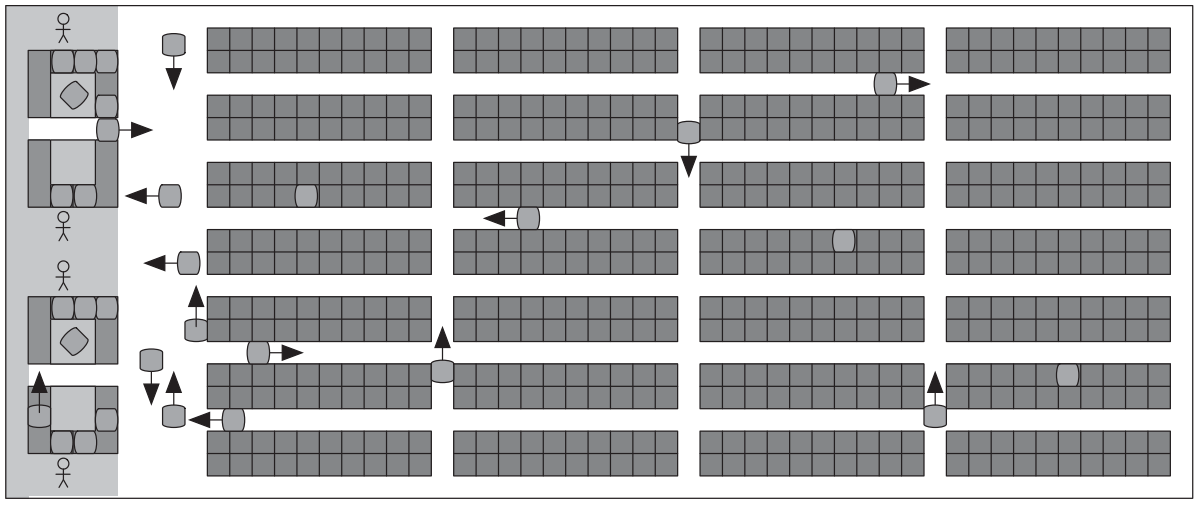
\includegraphics[width=0.9\textwidth]{graphics/kivasystemlayout}
	\caption{Kiva system representation on square grid map (\cite{wurman2008coordinating})}
	\label{fig:kivawarehouse}
\end{figure}

Different to traditional the MAPF problem, the objective of a Kiva system is mainly to minimize the downtime of human pickers. This requires the drive units to bring a steady supply of products to the order picker. Additionally Kiva systems run 24 hours a day hence the measures of makespan and sum of costs are not quite representative as they require a goal-state to be reached. For MAPF algorithms which were applied to a Kiva domain, we look at whether new objectives were used to measure performance.

\section{Suboptimal multi-agent pathfinding algorithms} \label{sec:suboptimal}
This section looks at suboptimal MAPF algorithms, here ware are mainly focused on makespan and scalability. As these will be helpful for comparison against opitmal MAPF algorithms.

%\begin{center}
%\begin{tikzpicture}
%\centering
%\draw[step=1cm,gray,very thin] (0,0) grid (5,3);
%\fill[gray!] (0,0) rectangle (3,1);
%\node at (0.5, 2.5) {$a_2$};
%\node at (0.5, 1.5) {$a_1$};
%\end{tikzpicture}
%\end{center}

\subsection{Cooperative A*}
Cooperative A* is a decentralized algorithm where a search is performed for one agent at a time, the resulting path is stored in a \textit{reservation table}. Subsequent agents must treat any stored paths in the reservation table as obstacles when performing their search. The reservation table is often stored as a matrix describing an agent is at a node $n$ at time $t$.

A variant of this is \textit{hierarchical cooperative A*} (HCA*) which relies on an algorithm called \textit{reverse resumable A*} in order to calculate a smarter heuristic. A variant of HCA*, \textit{windowed hierarchical cooperative A*} (WHCA*) restricts the time window of the reservation table for agents to query. During an agent's path, this window is updated and the agent will see more information in the reservation table. \cite{silver2005cooperative} defines HCA* and WHCA* and provides background of work on CA*.

Cooperative A* and HCA* do not scale well but WHCA* is found a solution in under 0.6 ms per agent and was suggested that it is usable in real-time. For solution quality, the average path length was calculated with the baseline being the shortest path ignoring other agents. WHCA* generally found a path $\frac{3}{2}$ longer than that of the shortest path (with 100 agents in the simulation). This gap scaled as the number of agents increased. WHCA* is often used a benchmarks of newer algorithms and but these algorithms often surpass it in runtime.

\newpage \subsection{MAPP}
MAPP (\cite{wang2011mapp}) is a suboptimal algorithm which has a polynomial runtime complexity and is complete for slidable problems. It finds a runtime complexity of $O(n^2k^2)$ where $n$ is the number of nodes on the graph and $k$ is the number of agents. It guarantees this by identifying sets of units which are guaranteed to run in polynomial time. A slidable problem is identified when there exists an $\Omega$ path for each agent as seen in Figure~\ref{fig:omegapath}.

% MAPP that it does not require replanning.

%\begin{figure}[H]
%	\centering
%	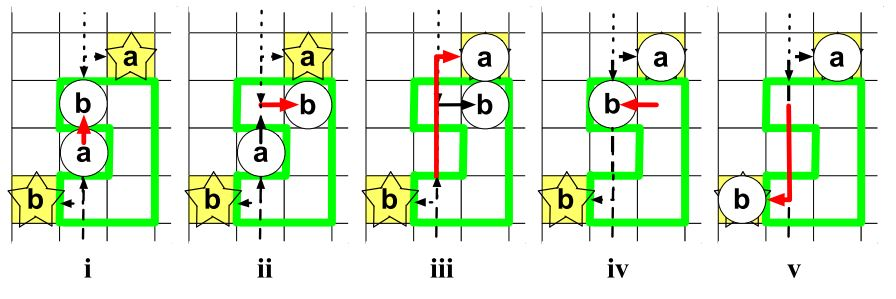
\includegraphics[width=\linewidth]{graphics/mappblank}
%	\label{fig:mappblank}
%	\caption{Example of how MAPP works (\cite{wang2011mapp})}
%\end{figure}

In comparison to FAR and WHCA*, MAPP excels in having high completeness at 92\%--99.7\%, compared to FAR (81.87\%) and WHCA* (80.87\%). Speed-wise, MAPP is comparable to WHCA* and 10 times slower than FAR  but in scenarios where MAPP has $\Omega$ paths, MAPP gains significant benefits and is only 2.18 times slower than FAR and 4.8--5.2 times faster than WHCA*.

\begin{figure}[H]
	\centering
	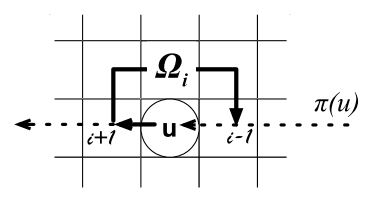
\includegraphics[width=0.4\linewidth]{graphics/omegapath}
	\caption{An example of an alternate path, $\Omega$ (\cite{wang2011mapp})}
	\label{fig:omegapath}
\end{figure}

It should be noted MAPP identifies the situation in which agents attempt to pass a tunnel as MAPP fails otherwise at this case. Their solution, called a \textit{buffer zone extension} is used and importantly it has little performance degrades, with the same runtime complexity as the regular MAPP algorithm and little additional memory requirements. This is relevant as MAPP would not function without in the narrow aisles of Kiva systems without this.

MAPP may be a desirable choice for use in Kiva systems as it scales up to 2000+ agents and is complete. Kiva systems often have high density of agents so MAPP would perform well in finding a solution compared alternative suboptimal algorithms (WHCA* and FAR).

\section{Optimal multi-agent pathfinding algorithms} \label{sec:optimal}
This section looks at three optimal MAPF algorithms, \textit{centralized A*}, \textit{conflict based search} and \textit{increasing cost search tree}. We focus on their approach to improving scalability and any applications to Kiva systems.

\subsection{Centralized A*}
Centralized A* is an optimal algorithm which is exponential in the number of agents. It uses a global heuristic usually the sum of individual costs\footnote{sum of individual costs: the sum of path distances when ignoring collisions with other agents} to lead towards the optimal solution. One recent variant \textit{enhanced partial A* expansion} (EPEA*) by \cite{goldenberg2014enhanced}, only generates children which have the same $f$-cost as their parent node.

Two algorithms, Independence Detection and Operator Decomposition help to reduce the number of agents being processed and hence provides an exponential speed up to Centralized A*. More details about ID and OD is described in Section~\ref{sec:generalimprovements}. Both EPEA* and A*+OD were previously state-of-the-art in optimal MAPF and are used as benchmarks for many other optimal MAPF algorithms.

\subsection{Conflict based search} \label{sec:cbs}
The conflict-based search algorithm (\cite{sharon2015conflict}) relies on building a binary tree known as a  \textit{constraint tree} (CT). Each node in the CT describes a set of constraints, a solution and the cost of this solution (Figure~\ref{fig:constraintree}). A constraint prohibits an agent $a$ from being at node $n$ at timestep $t$, in the form of $\langle a, n, t \rangle$.

\begin{figure}[!htb]
	\centering
	\centering
	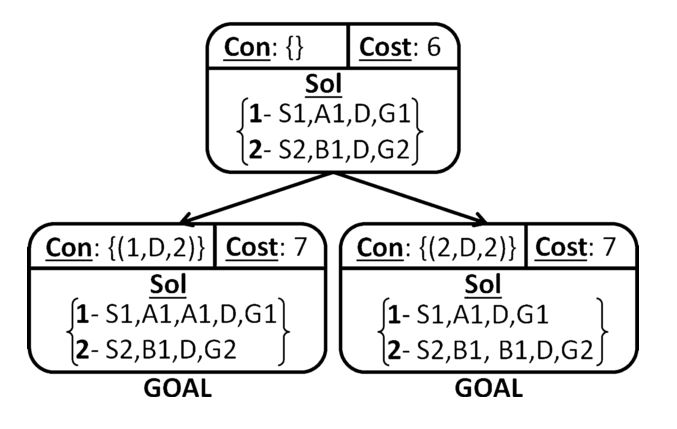
\includegraphics[width=0.5\linewidth]{graphics/constrainttree}
	\caption{An example of a Constraint Tree (CT) (\cite{sharon2015conflict})}
	\label{fig:constraintree}
\end{figure}

A node in the CT is processed by finding the shortest path for each agent to their goal making sure to satisfy the constraints described by the node. If this path is not valid and a collision has occurred between two agents: $a_1, a_2$ then CBS branches and adds two successor nodes. Both successors inherit the constraints of the parent node. Additionally the left successor will adds a new constraint $\langle a_1, n, t \rangle$ while the right successor will add the constraint $\langle a_2, n, t \rangle$. CBS is optimal as it chooses the next node to expand by searching for the lowest cost node in the CT.


As CBS branches at every conflict, it is exponential in the number of conflicts. In comparison to EPEA*, CBS performed worse in maps with open spaces where sets of agents are more likely to be \textit{strongly coupled}, that is they have a high rate of path conflicts between one another. On the other hand CBS was found to perform better in maps with bottlenecks.

\begin{figure}[!htb]
	\centering
	\centering
	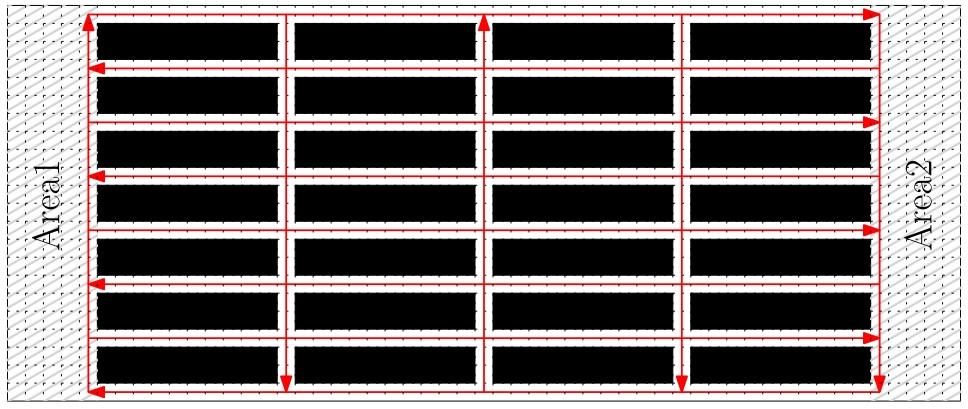
\includegraphics[width=0.9\linewidth]{graphics/ecbskivadomain}
	\caption{Kiva-like domain with Area1 on the LHS and Area2 on the RHS (\cite{cohen2016improved})}
	\label{fig:cbskivadomain}
\end{figure}


A bounded-suboptimal variant of CBS was developed called improved-ECBS (iECBS) \cite{cohen2016improved}. iECBS was tested on a Kiva system domain of size $22 \times 54$ with 130 agents (Figure~\ref{fig:cbskivadomain}). This test did not model the Kiva problem as described in Section~\ref{sec:problemdef}, instead the problem generated half the agents in \textit{Area1} and half the agents in \textit{Area2} of the map. Agents were then given the task of moving random goal location in the opposite area. Testing was performed against ECBS and found speedups in runtime of approximately 10 times. The scalability of iECBS was measured in this environment and found it performed reasonably at around 150-160 agents at a success rate of 90\% before dropping off. iECBS was not testing aginst CBS but ECBS was tested previously (\cite{barer2014suboptimal}). Here they used the DAO game map (BRC202) from \cite{sturtevant2012benchmarks} and found that CBS had a steep fall off in success rate at 20-25 agents as compared to ECBS at 130-140 agents. This is a significant increase in scalability and the user set parameter (\ref{sec:bsov}) for this test: $w = 1.01$ indicates the solution quality was near optimal.

%\begin{figure}[!htb]
%	\centering \tiny
%	\begin{minipage}{0.4\textwidth}
%	\centering
%	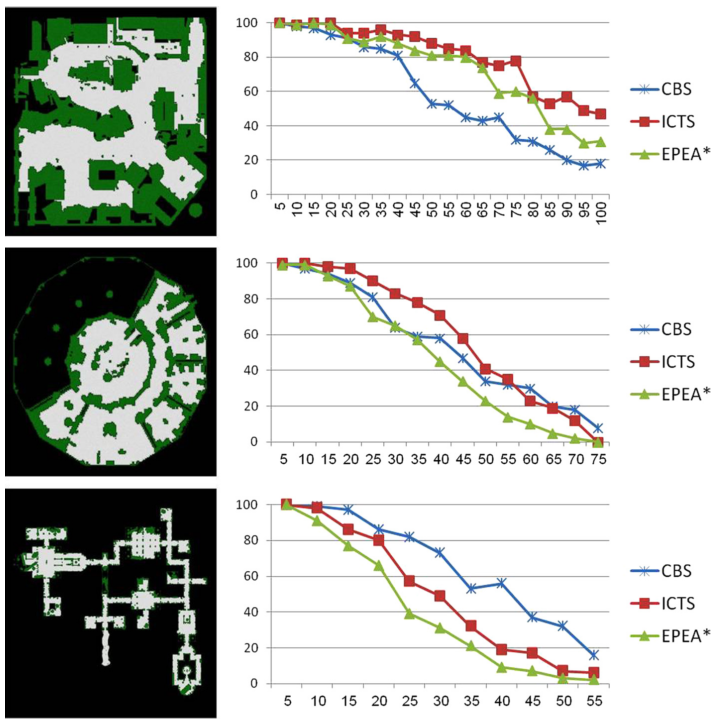
\includegraphics[width=\linewidth]{graphics/cbsresults1}
%	\caption{A Small Region of a Kiva Layout (\cite{sharon2015conflict}). Picking stations located on the left and storage pods laid out in rows.}
%	\label{cbsresults1}
%	\end{minipage}
%	\begin{minipage}{0.4\linewidth}
%		\centering
%	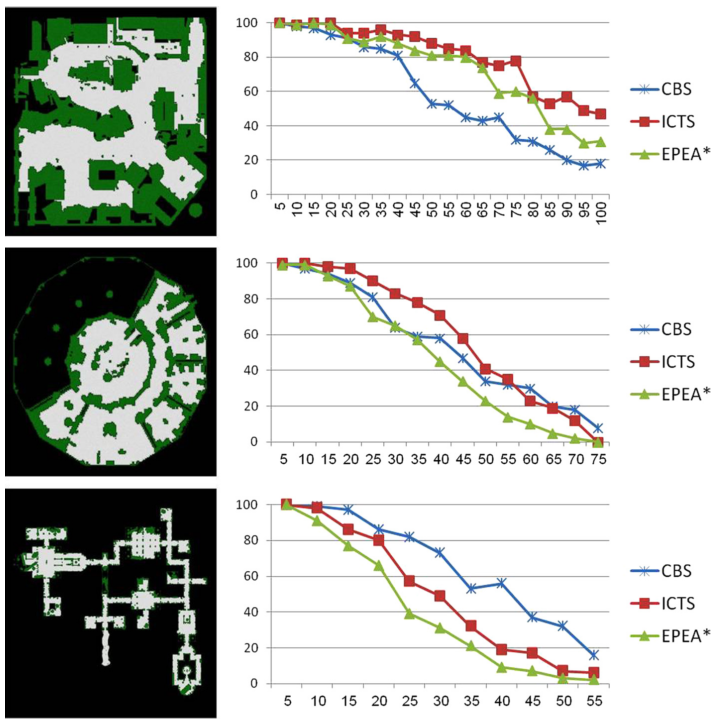
\includegraphics[width=\linewidth]{graphics/cbsresults1}
%	\caption{A Small Region of a Kiva Layout (\cite{sharon2015conflict}). Picking stations located on the left and storage pods laid out in rows.}
%	\label{cbsresults2}
%	\end{minipage}
%\end{figure}

%Here CBS was compared against ICTS, EPEA*.

\subsection{Increasing Cost Search Tree}
This section describes the Increasing Cost Search Tree (ICTS) an optimal, complete MAPF algorithm (\cite{sharon2011increasing}). The ICTS algorithm generates a tree known as an \textit{increasing cost tree} (Figure~\ref{fig:increasingcosttree}). Each node in the tree describes a cost $C$ for each agent $[C_1,\dots,C_k]$. ICTS generates paths based off the cost for each agent described in the node. It explores all permutations of paths which are equal to $C_i$ and a valid solution when a combination of paths is conflict-free.  To build the tree, the root starts containing the an optimal cost ignoring any collisions with other agents. When it does not find a valid solution, the algorithm will branch and generate $k$ successors, one for each agent. In each of the successors, the cost of $i$ will increment e.g. for successor 2: $[C_1,C_{2}+1,\dots,C_k]$. By exploring the tree in breadth-first manner, ICTS ends up with an optimal solution.

\begin{figure}[!htb]
	\centering
	\centering
	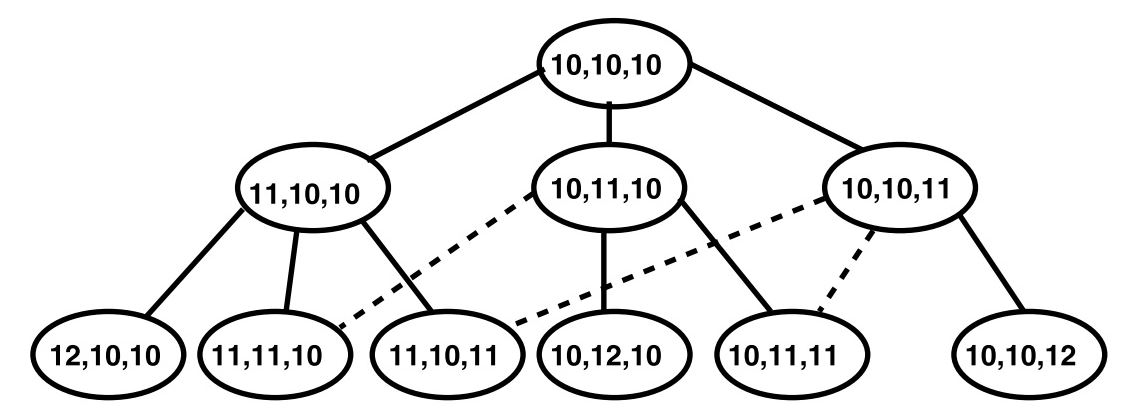
\includegraphics[width=0.9\linewidth]{graphics/ictstree}
	\caption{ICT for three agents (\cite{sharon2011increasing})}
	\label{fig:increasingcosttree}
\end{figure}

The ICT grows exponentially in $\Delta$, where delta is the difference between the optimal collision-free cost and the optimal cost which ignores collision (the root node). Hence the downfall of ICTS is an environment with many conflicts occurs or it is costly to resolve the conflicts, thus having a large $\Delta$. In comparison to $A*$ which is exponential in $k$, ICTS is exponential in $\Delta$ so it benefits most on open maps with many agents.

%\subsection{Integer Linear Programming}
%Integer Linear Programming (ILP) is an optimization technique. It looks at an objective function subject to a list of constraints and finds the optimal solution for each variable.
%
%\subsection{ILP (combined target-assignment and pathfinding)}
%\cite{ma2016optimal} covers the use of Network Flow, More details about the use of ILP is in Section~\ref{sec:tapf}.
%
%where agents are anonymous. 
%
%reduction to the integer multi- commodity flow problem on a time-expanded network.
%
%\cite{yu2016optimal} takes a Network Flow approach. The solver uses the branch-and-bound algorithm. Anytime approach.

%\subsection{ILP (Network Flow)}
%\cite{yu2013multi} connects multi-agent path planning on graphs (roadmaps) to network flow problems, showing that the former can be reduced to the latter, therefore enabling the application of combinatorial network flow algorithms, as well as general linear program techniques, to multiagent path planning problems on graphs.
%
%\cite{yu2016optimal} looks at Complete Algorithms and Effective Heuristics.
%
%\cite{yu2015optimal} looks at the Structure and Computational Complexity.

\subsection{Combined-target assignment and pathfinding} \label{sec:tapf}
This section describes the work by \cite{ma2016optimal}, which looks at developing MAPF algorithms for autonomous warehouse robots, they call this a combined assignment and pathfinding (TAPF) problem. Importantly the difference between a MAPF problem and a TAPF problem is that:

\begin{compactitem}
	\item Agents are split into teams and a team of $k$ agents will have $k$ goal locations
	\item Agents are \textit{anonymous}: the goal location is interchangeable for each agent, so any agent can be assigned to a goal to satisfy the MAPF problem
\end{compactitem}

An important property is that anonymous MAPF problems can be solved in polynomial time. Their paper describes two algorithms which are made to solve the TAPF problem. Both of these use a hierarchical approach with a high-level and a low-level algorithm. First is conflict-based min-cost flow (CBM), which uses CBS (\ref{sec:cbs}) at the high-level and a min-cost max-flow algorithm on the low-level. CBM is applied to Kiva Systems which is their motivation behind formulating the TAPF problem. Their problem instances for Kiva Systems contain 420 drive units moving to 7 picking stations, the total warehouse size was not stated. Results suggested that  was performed well enough to be used in real-world applications of Kiva systems, with an 80\% success rate, mean makespan of 63.83 seconds and mean running time of 91.61 seconds. Importantly the results beat that of bounded suboptimal MAPF algorithms which were designed for Kiva systems.

Next, ILP (TAPF), which is similar to CBM but instead of using CBS at the high level it uses an ILP-based TAPF solver is used at the low-level. This ILP solver is based off the work by (\cite{yu2013multi}) and uses a network-flow approach. Results found that this solver performed worse than the ILP MAPF solver in runtime and success rate but won in makespan.

Overall the formulation of the TAPF problem is beneficial in improving scalability between optimal and suboptimal algorithms and will be looked at in further work.

\section{Independence detection and operator decomposition} \label{sec:generalimprovements}
This section looks at two MAPF techniques developed by \cite{standley2010finding} which can be applied to most MAPF algorithms and provide significant speedups.

\noindent \textbf{Independence detection}. Independence detection (ID) finds independent groups of agents where it can be proven for each of these groups that the agents within them will not be in conflict. These groups are split and treated as seperate subproblems. Importantly this reduces the number of agents and provides an exponential speed up for A* and a polynomial speedup for many non-A* based algorithms.

\noindent \textbf{Operator decomposition}. Operator decomposition (OD) reduces the branching factor by performs one agent's action at a time as oppose to an operator applying to every agent simultaneously. OD gives a much deeper tree but with a much smaller branching factor. At every $k$ levels in the tree we get an equivalent state where OD would not be used and hence the branching factor can be seen as $a$ instead of $a^k$ where $a$ is the number of possible actions and $k$ is the number of agents.

\cite{standley2010finding} found that OD had larger benefits and scaled better than ID but they can both be used in conjunction.

\newpage

\section{Discussion} \label{sec:discussion}

\begin{table}[ht]
	\centering
	\small
	\begin{tabular}{ l c c c c c p{2.3cm}}
		
		\textbf{Name} & \textbf{BSV} & \textbf{Complete} & \textbf{Complexity} & \textbf{KS} & \textbf{Comparison} \\
		\hline
		\multicolumn{6}{l}{\textbf{Optimal}} \\
		\hline
		CBS 				& N & Y & Exp conflicts & Y & ICTS, EPEA* \\
		Centralized A* 		& Y & Y & Exp agents & N & -- \\
		ICTS 				& Y & Y & Exp $\Delta$ & N & A*, A*+OD \\
		ILP	(TAPF)			& N & Y & Poly conflicts & N & ILP (NF)\footnote{ILP using Network Flow (\cite{yu2013multi})}, IPL (TAPF) \\
		CBM 				& N & Y & Poly conflicts & Y & ILP (NF), IPL (TAPF) \\
		\hline
		\multicolumn{6}{l}{\textbf{Suboptimal}} \\
		\hline
		MAPP 				& N & Y & Poly agents, nodes & N & WHCA*, FAR\footnote{Flow Annotation Replanning (\cite{wang2008fast})} \\
		WHCA* 				& N & N & Poly agents & N & -- \\
	\end{tabular}

	\caption{Table comparing the stated algorithms and their properties. \textbf{BSV}: Does the algorithm have a bounded-suboptimal variant. \textbf{Complexity}: Runtime complexity. \textbf{KS}: has the algorithm been applied to Kiva systems. \textbf{Comparision}: the algorithms used for benchmark testing.}
	\label{table:comparison}
\end{table}

In regards to suboptimal algorithms, none were applied to Kiva systems. It would be useful to see the relative performance between suboptimal solutions and optimal solutions within a Kiva system domain. MAPP seems a good choice for comparison against optimal MAPF algorithms. It is far from optimal but is complete and this is especially relevant to Kiva systems where the environment is dense with agents. Other suboptimal algorithms (FARR, WHCA*) would likely fail to find a solution in these situations.

We found that optimal algorithms can improve scalability by relaxing the solution quality and creating a bounded-suboptimal variant. Two examples of these are iECBS~(\cite{cohen2016improved}) and EPEA*~(\cite{goldenberg2014enhanced}). In the case of CBS, this approach increase the scalability of the optimal algorithm by a factor of around 6 times. Hence allowing for a solution to be found with 85\% success rate on the DAO game map (BRC202), populated with 200 agents.

Another approach to improving scalability, \cite{ma2016optimal} finds large gains in defining a special case of the MAPF problem, the TAPF problem which applies to Kiva systems. The important difference here is that agents are anonymous. Their algorithm, CBM takes advantage of this formulation and is an optimal algorithm that can scale up to 450 agents with 80\% success rate. This optimal algorithm wins over even the bounded-suboptimal variants of CBS. 

This is an important development and it would be interesting to see if a bounded-suboptimal variant of CBM can be made and if the variant will provide benefits on the same scale as iECBS gives to CBS.  This gap seems like a good fit for our work and we look at these two techniques and applying them together, possibly scaling up to the 1000+ agents required by Kiva systems.

In literature which look at Kiva systems, iECBS (\cite{cohen2016improved})  and CBM (\cite{ma2016optimal}), the downtime of human pickers is overlooked. In the case of CBM the algorithm takes a snapshot of the system and performs one cycle of the Kiva process. For ECBS, the algorithm simply looked at a Kiva-like environment and moved agents from one side to the other. For both papers, the objective was on makespan and success rate. Unlike the approach where CBM looks at snapshotting a instance of the Kiva system problem, we may look at generating a fixed number of orders and seeing how long the simulation takes to fulfill these orders, the sum of costs and the downtime. This approach would allow for future work in modelling the other problems within Kiva systems as described in Section~\ref{sec:introduction}.

In conclusion, we will be aiming formulate the Kiva system problem as a TAPF problem and begin by taking an optimal approach. A bounded-suboptimal variant will be developed to further improve scalability. We expect to be able to scale to equivalent scales as in CBM (450 agents) and possibly up to 1000+ agents with the combination of a bounded-suboptimal variant. Finally we hope to see the consequences when the downtime of the system is the objective.

%Lastly, another motivation to looking into the objective of downtime: an optimal algorithm would allow for shorter paths to be found compared to a suboptimal algorithm hence less agents are required to fulfill the same supply of inventory. As less agents are required in the simulation, the complexity of the MAPF problem is reduced. Therefore there may be a balance of adjusting the solution quality to provide more efficient agents thus keeping the same supply of inventory, while reducing the complexity. We hope to look at this relation in detail and perhaps find a point where it is better to simply add more agents to increase supply or increase the efficiency of each agent.

\bibliographystyle{dcu}
\bibliography{bibliography}
	
\end{document}
